\section{向量和数学数组}
向量是数据的集合。 向量很有用,因为计算机中的并行性来自计算机硬件的集合,
并且数据通常在相关分组中进行处理(例如,RGB 像素中的颜色通道)。 
这个概念非常重要,因此我们花了一章的时间讨论不同的 SYCL 向量类型以及如何使用它们。 
请注意,本章中我们不会深入讨论标量运算的向量化,因为这会根据设备类型和实现而有所不同。 第 16 章介绍了标量运算的向量化。

本章旨在解决以下问题:

\begin{itemize}
	\item 什么是向量类型?

	\item SYCL 数学数组(marray) 和向量(vec) 类型之间有什么区别?

	\item 我应该何时以及如何使用marray 和vec?
\end{itemize}

我们使用工作代码示例讨论 marray 和 vec,并重点介绍利用这些类型的最重要方面。

\subsection{向量类型的歧义}
当我们与并行编程专家交谈时,向量是一个令人惊讶的有争议的话题。 
根据作者的经验,这是因为不同的人以不同的方式定义和思考向量。

有两种广泛的方式来思考本章所说的向量类型:

\begin{enumerate}
	\item 作为一种便捷类型,它将我们可能想要引用和操作的数据分组为一组,例如像素的 RGB 或 YUV 颜色通道。 
	我们可以定义一个像素类或结构,并在其上定义像 + 这样的数学运算符,但便利类型可以开箱即用地为我们做到这一点。 
	在许多用于对 GPU 进行编程的着色器语言中都可以找到便利类型,因此这种思维方式在许多 GPU 开发人员中很常见。

	\item 作为描述代码如何映射到硬件中的SIMD(单指令,多数据)指令集的机制。 
	例如,在某些语言和实现中,float8 上的操作可以映射到硬件中的八通道 SIMD 指令。 
	SIMD 向量类型在许多语言中用作 CPU 特定内联函数的高级替代方案,因此这种思维方式在许多 CPU 开发人员中已经很常见。
\end{enumerate}

尽管这两种对向量类型的解释非常不同,但随着 SYCL 和其他语言同时适用于 CPU 和 GPU,它们无意中结合在一起并混在一起。 
vec 类(存在于 SYCL 1.2.1 中,并且仍然存在于 SYCL 2020 中)与任一解释兼容,
而 marray 类(在 SYCL 2020 中引入)被明确描述为与 SIMD 矢量硬件指令无关的便利类型 。

\begin{remark}[变化即将到来:SIMD 类型]
SYCL 2020 尚未包含与第二种解释(SIMD 映射)明确相关的向量类型。
但是,已经有一些扩展允许我们编写显式向量代码,这些代码直接映射到硬件中的 SIMD 指令,
专为想要为特定架构调整代码并从编译器矢量器中获取控制权的专家程序员而设计。
我们还应该期望另一种向量类型最终出现在SYCL中,以涵盖第二种解释,
可能与建议的C++ std::simd模板一致。这个新类将非常清楚地说明代码何时以显式向量样式编写,以减少混淆。
SYCL 中现有的扩展和未来的类似 std::simd 的类型都是我们预计很少有开发人员使用的利基功能。

有了 marray 和专用的 SIMd 类,我们作为程序员的意图将从我们编写的代码中清晰可见。
这样就不那么容易出错,不那么容易混淆,甚至可能减少专家开发人员之间在出现“什么是向量”问题时激烈讨论的次数。
\end{remark}

\subsection{我们对于 SYCL 向量类型的心智模型}
在本书中,我们讨论了如何将Work-Items分组在一起以公开强大的通信和同步原语,例如Sub-Group屏障和洗牌。 
为了使这些操作在向量硬件上高效,需要假设Sub-Group中的不同Work-Items组合并映射到 SIMD 指令。 
换句话说,多个Work-Items由编译器组合在一起,此时它们可以映射到硬件中的 SIMD 指令。 
请记住第 4 章中的内容,这是在矢量硬件之上运行的 SPMD(单程序、多数据)编程模型的基本前提,
其中单个Work-Items构成硬件中可能是 SIMD 指令的通道,而不是 定义整个操作的Work-Items,该操作将成为硬件中的 SIMD 指令。 
当映射到硬件中的 SIMD 指令、以 SPMD 风格编程时,您可以将编译器视为始终跨Work-Items进行向量化。

对于来自没有向量类型的语言或来自 GPU 着色语言的开发人员,
我们可以将 SYCL 向量类型视为Work-Items的本地向量类型,因为如果添加两个四元素向量,
则添加 可能需要硬件中的四个指令(从Work-Items的角度来看它将被标量化)。 
向量的每个元素将由硬件中的不同指令/时钟周期相加。 
这与我们对向量类型的解释是一致的——为了方便,我们可以在源代码中的单个操作中添加两个向量,
而不是在源代码中执行四个标量操作。

对于具有 CPU 背景的开发人员来说,我们应该知道 SIMD 硬件的隐式向量化在许多编译器中默认发生,与向量类型的使用无关。 
编译器可以跨Work-Items执行这种隐式向量化,从格式良好的循环中提取向量运算,
或者在映射到向量指令时尊重向量类型 - 有关更多信息,请参阅第 16 章。

本章的其余部分重点介绍如何使用向量类型(对于 marray 和 vec)的方便解释来教授向量,
这是我们在 SYCL 中编程时应该牢记的一点。

\begin{remark}[其他实现的可能!]
从理论上讲,SYCL 的不同编译器和实现可以对代码中的向量数据类型如何映射到 SIMD 向量硬件指令做出不同的决策。
我们应该阅读供应商的文档和优化指南,以了解如何编写映射到高效 SIMD 指令的代码,
尽管本章中描述的思维和编程模式适用于大多数(理想情况下是所有)SYCL 实现。
\end{remark}

\subsection{数学数组 (marray)}
\begin{figure}[H]
	\centering
	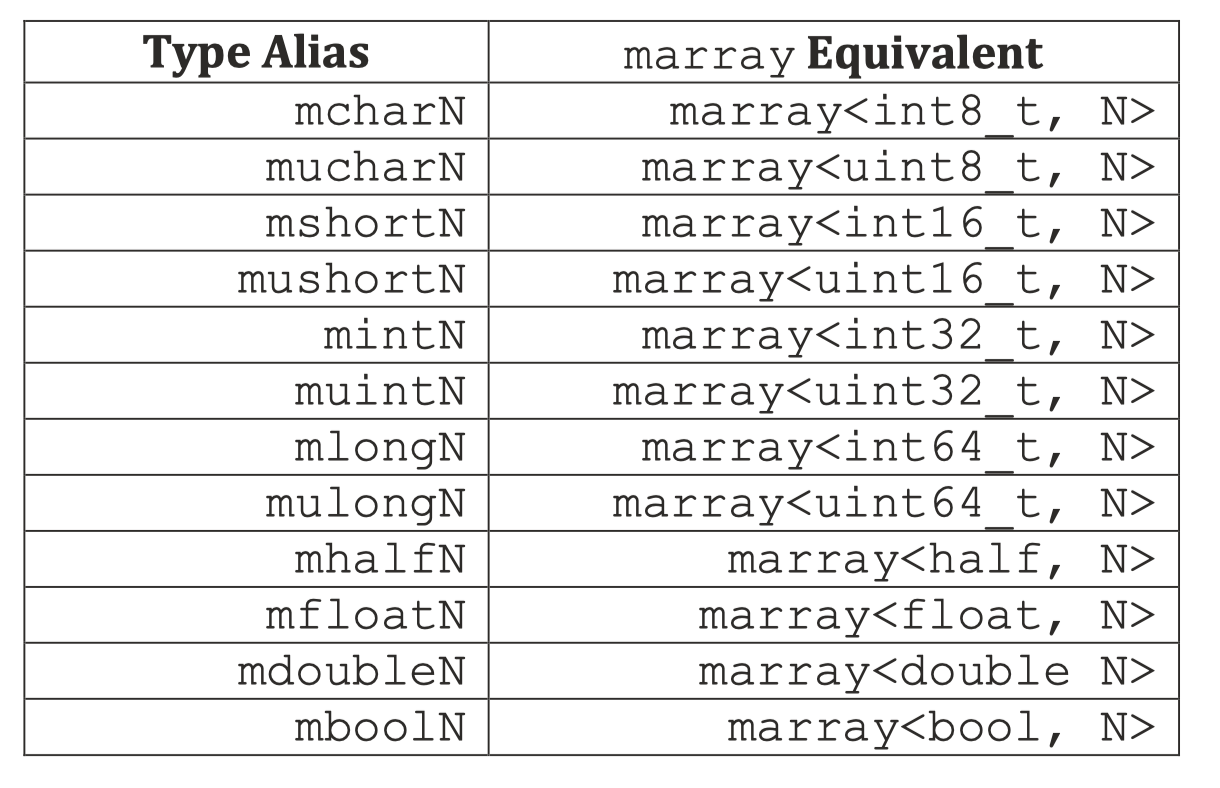
\includegraphics[width=0.9\textwidth]{figs/F11.1.png}
	\caption{\textit{数学数组的类型别名 }}
\end{figure}

SYCL 数学数组类型 (marray),请参见图 11-1,是 SYCL 2020 中的新增内容,
其定义是为了消除对向量类型应如何表现的不同解释的歧义。 
marray 显式地表示了本章上一节中介绍的向量类型的第一种解释——与向量硬件指令无关的便利类型。 
通过从名称中删除“向量”并包含“数组”,可以更轻松地记住和推理类型如何在硬件上逻辑实现。

marray 类根据其元素类型和元素数量进行模板化。 
元素数量参数 NumElements 是一个正整数 — 当 NumElements 为 1 时,数组可以隐式转换为等效的标量类型。 
元素类型参数 DataT 必须是 C++ 定义的数值类型。

Marray 是一个数组容器,与 std::array 类似,
还额外支持数组上的数学运算符(例如 +、+=)和 SYCL 数学函数(例如 sin、cos)。 
它旨在为 SYCL 设备上的并行计算提供高效且优化的数组操作。

为了方便起见,SYCL 为数学数组提供了类型别名。 
对于这些类型别名,元素数量 N 必须为 2、3、4、8 或 16。

\begin{figure}[H]
	\centering
	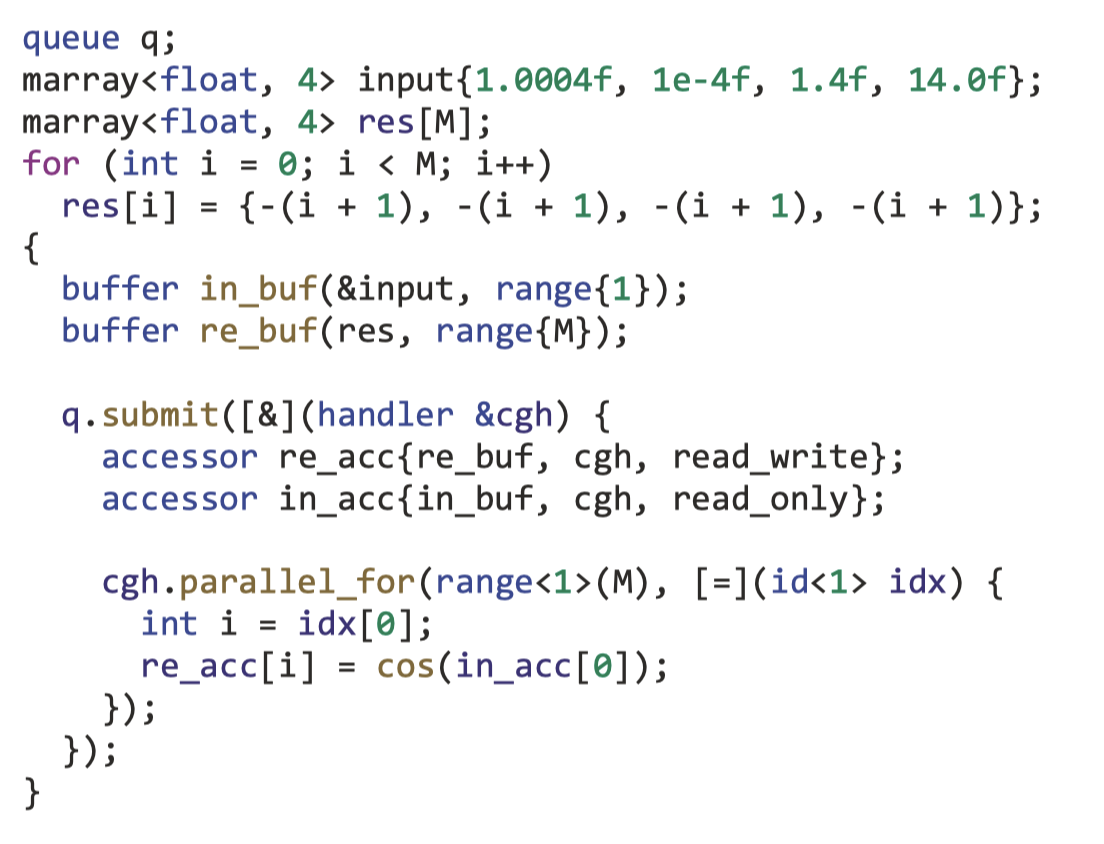
\includegraphics[width=0.9\textwidth]{figs/F11.2.png}
	\caption{\textit{使用 marray 的简单示例 }}
\end{figure}

图 11-2 显示了如何将 cos 函数应用于由四个浮点数组成的数组中的每个元素的简单示例。 
此示例强调了使用数组来表达适用于分配给每个Work-Items的数据集合的所有元素的操作的便利性。

通过在大范围的数据 M 上执行该Kernel,我们可以在许多不同类型的设备上实现良好的并行性,
包括那些比数组的四个元素宽得多的设备,而无需规定我们的代码如何映射到 SIMD 指令集操作 关于向量类型。

\subsection{矢量(vec)}
SYCL 向量类型 (vec) 存在于 SYCL 1.2.1 中,并且仍包含在 SYCL 2020 中。
如前所述,vec 与向量类型的任一解释兼容。 
在实践中,vec 通常被解释为一种方便类型,因此我们建议使用 marray 来提高代码可读性并减少歧义。 
但是,此建议有三个例外,我们将在本节中介绍:矢量加载和存储、与后端本机矢量类型的互操作性以及称为“swizzles”的操作。

与 marray 一样,vec 类根据其元素数量和元素类型进行模板化。 
但是,与 marray 不同的是,NumElements 参数必须为 1、2、3、4、8 或 16,任何其他值都会导致编译失败。 
这是一个很好的例子,说明了向量类型的混乱影响了 vec 的设计:将向量的大小限制为 2 的小幂对于 SIMD 指令集是有意义的,
但从寻求便利类型的程序员的角度来看似乎是任意的。 元素类型参数 DataT 可以是设备代码中支持的任何基本标量类型。

此外,与 marray 一样,vec 公开 2、3、4、8 和 16 个元素的简写类型别名。 
marray 别名以“m”为前缀,而 vec 别名则不然,例如,uint4 是 vec<uint32\_t, 4> 的别名,
float16 是 vec<float, 16> 的别名。 
在处理向量类型时,我们必须密切注意这个“m”的存在或不存在,以确保我们知道我们正在处理哪个类,这一点很重要。

\subsubsection{加载和存储}
vec 类提供用于加载和存储向量元素的成员函数。 这些操作作用于存储与向量通道相同类型的对象的连续内存位置。

\begin{figure}[H]
	\centering
	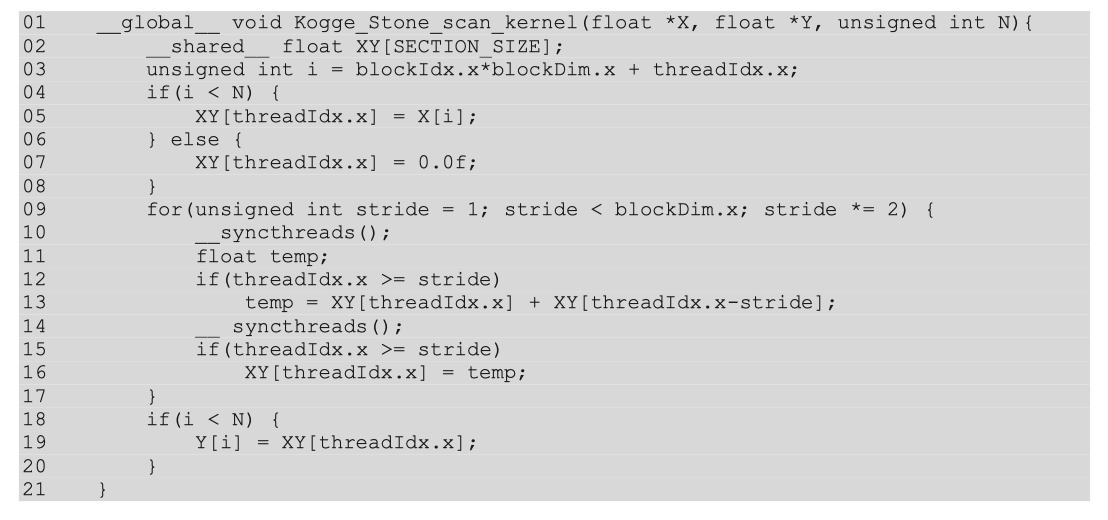
\includegraphics[width=0.9\textwidth]{figs/F11.3.png}
	\caption{\textit{vec 加载和存储功能 }}
\end{figure}

加载和存储函数如图 11-3 所示。 
load 成员函数从 multi\_ptr 地址处的内存中读取 DataT 类型的值(偏移量为 NumElements * DataT 的 offset 元素),
并将这些值写入 vec 的通道。 store 成员函数读取 vec 的通道,
并将这些值写入 multi\_ptr 地址处的内存,偏移量为 NumElements * DataT 的 offset 元素。

请注意,该参数是 multi\_ptr,而不是访问器或原始指针。 
multi\_ptr的数据类型是DataT,即vec类特化的组件的数据类型。 
这要求传递给 load 或 store 的指针必须与 vec 实例本身的组件类型匹配。

\begin{figure}[H]
	\centering
	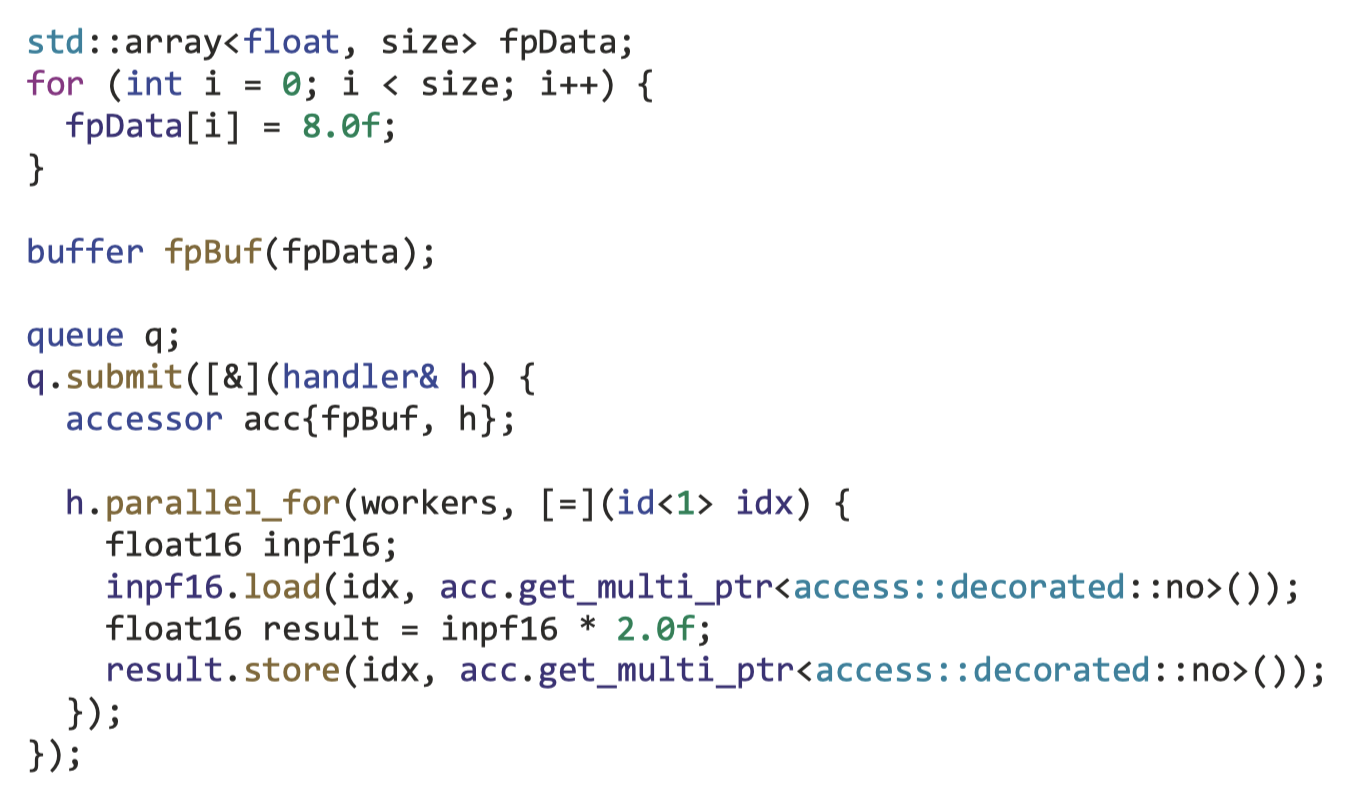
\includegraphics[width=0.9\textwidth]{figs/F11.4.png}
	\caption{\textit{使用 load 和 store 成员函数 }}
\end{figure}

图 11-4 显示了使用加载和存储函数的简单示例。

SYCL 向量加载和存储函数提供了用于表达向量运算的抽象,但底层硬件架构和编译器优化将决定任何实际的性能优势。 
我们建议使用分析工具分析性能并尝试不同的策略,以找到特定用例的向量加载和存储操作的最佳利用率。

尽管我们不应该期望向量加载和存储操作映射到 SIMD 指令,但使用向量加载和存储函数仍然有助于提高内存带宽利用率。 
有效地对向量类型进行操作向编译器暗示每个Work-Items正在访问连续的内存块,
并且某些设备可能能够利用此信息一次加载或存储多个元素,从而提高效率。

\subsubsection{与后端本机向量类型的互操作性}
SYCL vec 类模板还可以提供与后端的本机向量类型(如果存在)的互操作性。 
后端本机向量类型由成员类型 vector\_t 定义,并且仅在设备代码中可用。 
vec 类可以从 vector\_t 的实例构造,并且可以隐式转换为 vector\_t 的实例。

我们大多数人永远不需要使用 vector\_t,因为它的用例非常有限; 
它的存在只是为了允许与从Kernel函数内调用的后端本机函数进行互操作
(例如,从 SYCL Kernel内调用用 OpenCL C 编写的函数)。

\subsubsection{Swizzle 操作}
在图形应用程序中,混合意味着重新排列向量的数据元素。 
例如,如果向量 a 包含元素 {1, 2, 3, 4},并且知道四元素向量的分量可以称为 {x, y, z, w},
我们可以写成 b = a.wxyz(),向量 b 中的值为 {4, 1, 2, 3}。 
这种语法在代码紧凑性和具有用于此类操作的高效硬件的应用程序中很常见。

\begin{figure}[H]
	\centering
	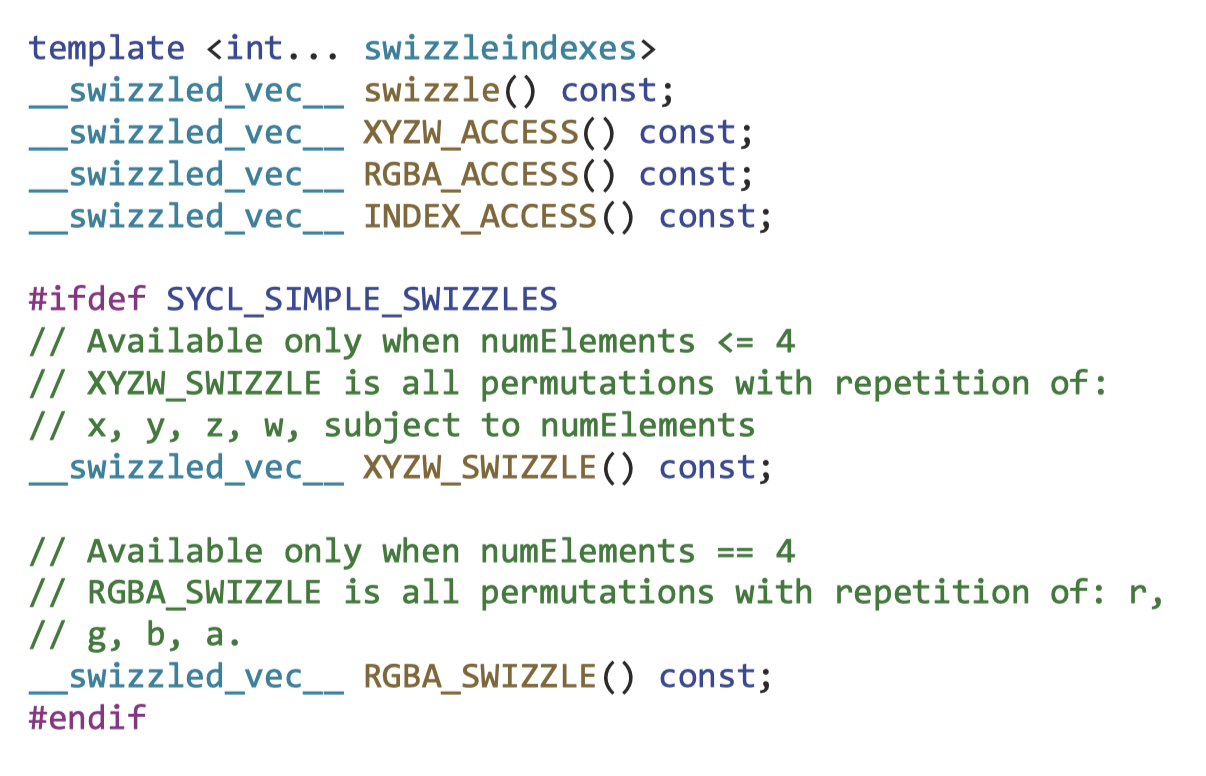
\includegraphics[width=0.9\textwidth]{figs/F11.5.png}
	\caption{\textit{vec swizzle 成员函数 }}
\end{figure}

vec 类允许以两种方式之一执行混合,如图 11-5 所示。

swizzle成员函数template允许我们通过调用模板成员函数swizzle来执行swizzle操作。 
此成员函数采用可变数量的整数模板参数,其中每个参数表示向量中相应元素的 swizzle 索引。 
swizzle 索引必须是 0 到 NumElements-1 之间的整数,
其中 NumElements 表示原始 SYCL 向量中的元素数量(例如,vec.swizzle<2, 1, 0, 3>() 表示四个元素的向量)。 
swizzle 成员函数的返回类型始终是 \_\_swizzled\_vec\_\_ 的实例,它是表示 swizzle 向量的实现定义的临时类。 
请注意,调用 swizzle 时不会立即执行 swizzle 操作。 
相反,当在表达式中使用返回的 \_\_swizzled\_vec\_\_ 实例时,会执行 swizzle 操作。

简单的 swizzle 成员函数集(在 SYCL 规范中描述为 XYZW\_SWIZZLE 和 RGBA\_SWIZZLE)
是作为执行 swizzle 操作的替代方法提供的。 这些成员函数仅适用于最多具有四个元素的向量,
并且仅当 SYCL\_SIMPLE\_SWIZZLES 宏在任何 SYCL 头文件之前定义时才可用。 
简单的 swizzle 成员函数允许我们使用名称 {x, y, z, w} 或 {r, g, b, a} 引用向量的元素,
并通过使用这些元素名称调用成员函数来执行 swizzle 操作 直接地。

例如,简单的 swizzles 启用之前使用的 XYZW swizzle 语法 a.wxyz()。 
通过编写 a.argb(),可以使用 RGBA swizzles 等效地执行相同的操作。 
使用简单的 swizzles 可以生成更紧凑的代码,并且与其他语言(尤其是图形着色语言)更匹配的代码。 
当向量包含 XYZW 位置数据或 RGBA 颜色数据时,简单的混合也可以更好地表达程序员的意图。 
简单 swizzle 成员函数的返回类型也是 \_\_swizzled\_vec\_\_。 
与 swizzle 成员函数模板一样,当在表达式中使用返回的 \_\_swizzled\_vec\_\_ 实例时,将执行实际的 swizzle 操作。

\begin{figure}[H]
	\centering
	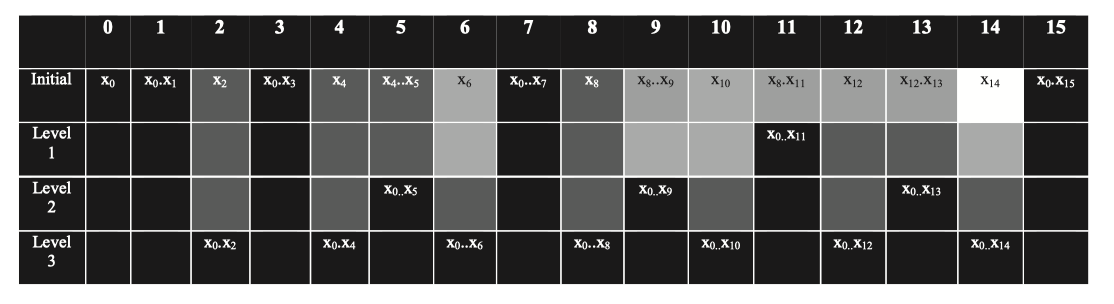
\includegraphics[width=0.9\textwidth]{figs/F11.6.png}
	\caption{\textit{使用 \_\_swizzled\_vec\_\_ 类的示例 }}
\end{figure}

图 11-6 演示了简单 swizzles 和 \_\_swizzled\_vec\_\_ 类的用法。 
虽然 \_\_swizzled\_vec\_\_ 没有直接出现在我们的代码中,
但它在 b.xyzw() * sw.wzyx() 等表达式中使用:b.xyzw() 和 sw.wzyx() 的返回类型
是 \_\_swizzled\_vec\_\_ 的实例, 并且直到结果被分配回 float4 变量 sw 后才会计算乘法。

\subsection{向量类型如何执行}
正如本章所述,向量类型及其如何映射到硬件有两种不同的解释。 到目前为止,我们特意只在高层讨论这些映射。 
在本节中,我们将更深入地研究向量类型的不同解释如何映射到 SIMD 寄存器等低级硬件功能,
证明这两种解释都可以有效利用向量硬件。

\subsubsection{向量作为便利类型}
关于向量如何从便利类型(例如,marray 和通常的 vec)映射到硬件实现,我们需要解决三个主要问题:

\begin{enumerate}
	\item 为了利用 SPMD 编程模型的可移植性和表现力,我们应该考虑组合多个Work-Items来创建向量硬件指令。 
	更具体地说,我们不应该认为向量硬件指令是从单个Work-Items中孤立创建的。

	\item 作为(1)的结果,从一个Work-Items的角度来看,
	我们应该将向量上的操作(例如加法)视为按时间执行每个通道或每个元素。 
	在我们的源代码中使用向量通常与利用底层向量硬件指令无关。

	\item 如果我们以某些方式编写代码(例如将向量的地址传递给函数),
	则编译器需要遵守向量和数学数组的内存布局要求,这可能会导致令人惊讶的性能影响。 
	了解这一点可以更轻松地编写编译器可以积极优化的代码。
\end{enumerate}

我们将从进一步描述前两点开始,因为清晰的思维模型可以使编写代码变得更加容易。

如第 4 章和第 9 章所述,Work-Items是并行层次结构的叶节点,代表Kernel函数的单个实例。 
Work-Items可以按任何顺序执行,并且不能相互通信或同步,
除非通过对本地或全局内存的原子内存操作,或通过组集合函数(例如,select\_from\_group、group\_barrier)。

便利类型的实例对于单个Work-Items来说是本地的,因此可以被认为相当于每个Work-Items的私有 NumElements 数组。 
例如,float4 y4 声明的存储可以被认为等同于 float y4[4]。 考虑图 11-7 中所示的示例。

\begin{figure}[H]
	\centering
	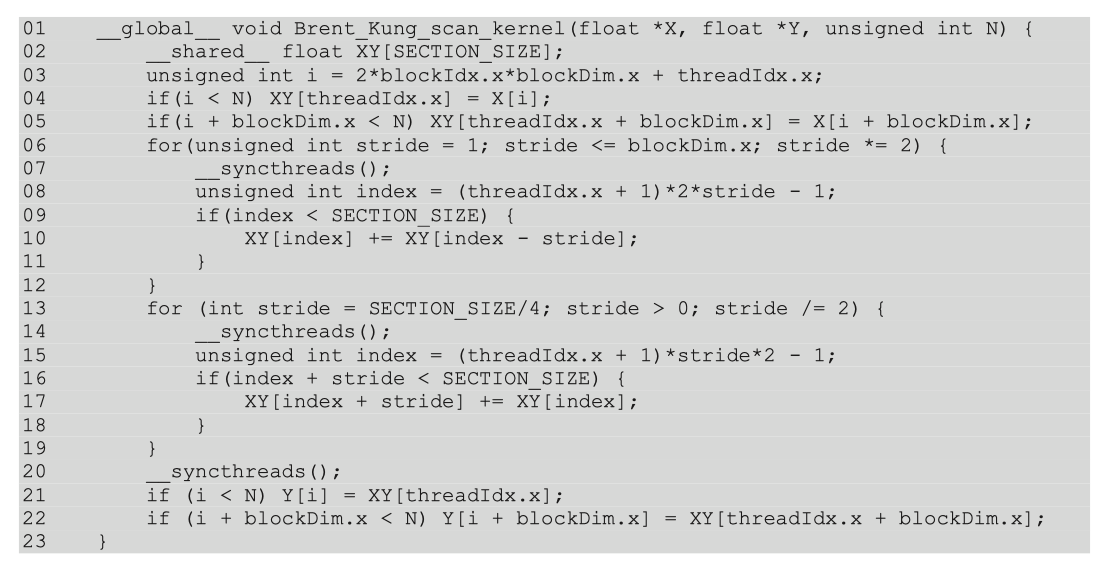
\includegraphics[width=0.9\textwidth]{figs/F11.7.png}
	\caption{\textit{向量执行示例 }}
\end{figure}

对于标量变量 x,在具有 SIMD 指令(例如 CPU、GPU)的硬件上使用多个Work-Items执行Kernel的结果
可能会使用向量寄存器和 SIMD 指令,但向量化是跨Work-Items的,并且与任何Work-Items无关。 
我们代码中的向量类型。 每个Work-Items都有自己的标量 x,可以在编译器生成的隐式 SIMD 硬件指令中形成不同的通道,
如图 11-8 所示。 在某些实现和某些硬件上,
Work-Items中的标量数据可以被认为是跨恰好同时执行的Work-Items隐式矢量化(组合成 SIMD 硬件指令),
但是Work-Items代码 我们编写的代码不会以任何方式对其进行编码——这是 SPMD 编程风格的核心。

以与硬件无关的方式暴露潜在的并行性可确保我们的应用程序可以扩展(或缩小)以适应不同平台的功能,
包括具有矢量硬件指令的平台。 
在应用程序开发过程中,在Work-Items和其他形式的并行性之间取得适当的平衡是我们所有人都必须面对的挑战,
第 15、16 和 17 章对此进行了更详细的介绍。

\begin{figure}[H]
	\centering
	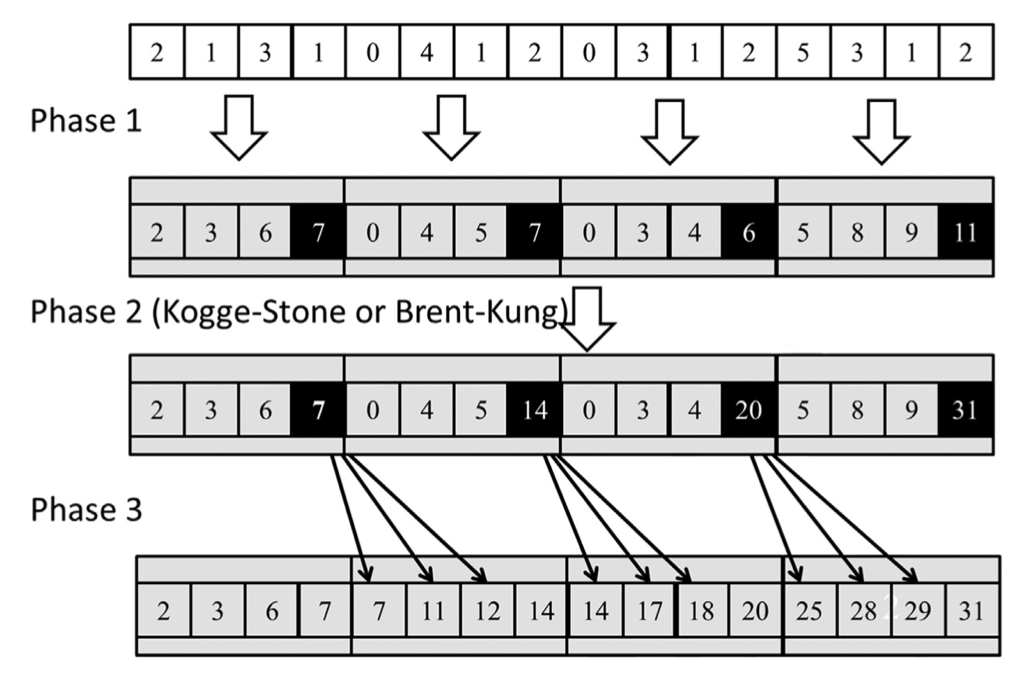
\includegraphics[width=0.9\textwidth]{figs/F11.8.png}
	\caption{\textit{从标量 x 到八位宽的硬件向量指令的可能扩展 }}
\end{figure}

通过编译器将标量变量 x 隐式向量扩展为向量硬件指令(如图 11-8 所示),
编译器根据多个Work-Items中发生的标量操作在硬件中创建 SIMD 操作。

回到图11-7的代码示例,对于向量变量y4,
多个Work-Items(例如8个Work-Items)的Kernel执行结果并没有使用硬件中的向量运算来处理四元素向量。 
相反,每个Work-Items独立地看到自己的向量(在本例中为 float4),并且对该向量元素的操作可能会跨多个时钟周期/指令发生。 
如图 11-9 所示。 我们可以将向量视为已由编译器从Work-Items的角度进行标量化。

\begin{figure}[H]
	\centering
	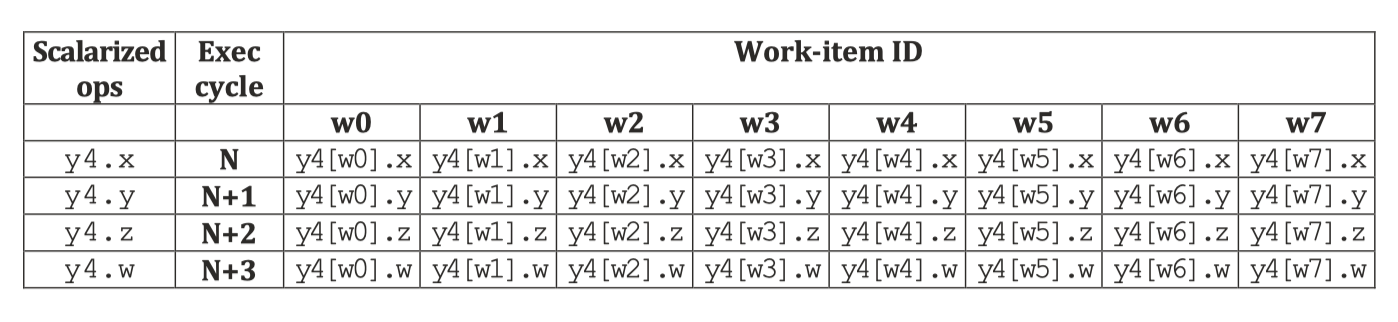
\includegraphics[width=0.9\textwidth]{figs/F11.9.png}
	\caption{\textit{硬件向量指令访问间隔的SIMD内存位置 }}
\end{figure}

图 11-9 还演示了本节的第三个关键点,即向量的方便解释可能会产生内存访问的影响,理解这一点很重要。 
在前面的代码示例中,每个Work-Items都会看到 y4 的原始(连续)数据布局,它提供了一个直观的模型来推理和调整。

\begin{figure}[H]
	\centering
	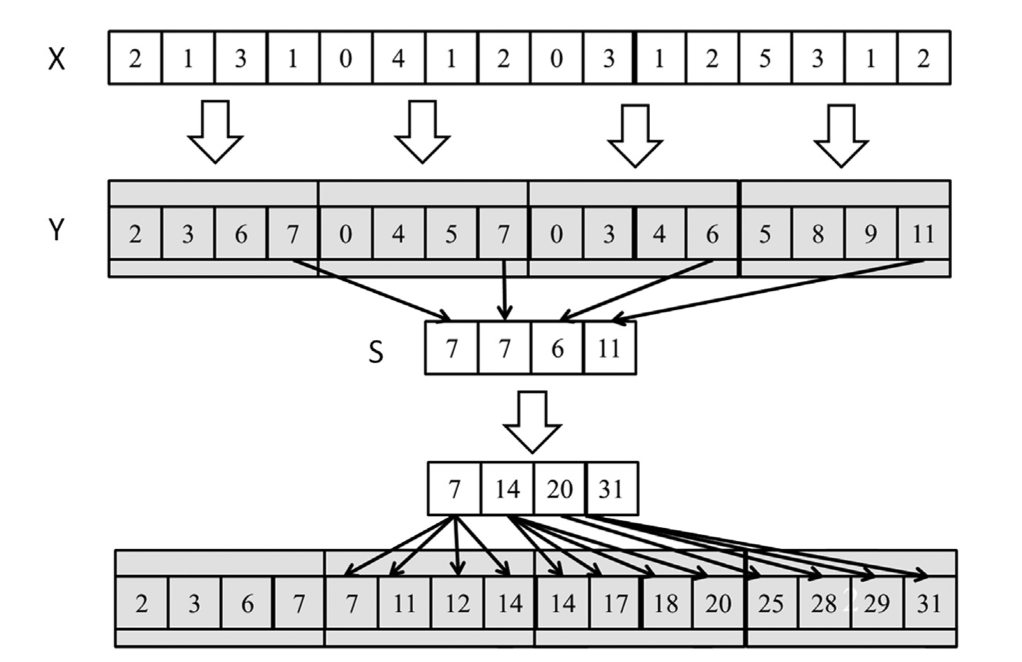
\includegraphics[width=0.9\textwidth]{figs/F11.10.png}
	\caption{\textit{具有地址转义的矢量代码示例 }}
\end{figure}

从性能角度来看,这种以Work-Items为中心的向量数据布局的缺点是,如果编译器跨Work-Items进行向量化以创建向量硬件指令,
则向量硬件指令的通道不会访问连续的内存位置。 取决于矢量数据大小和特定设备的功能; 
编译器可能需要生成、收集或分散内存指令; 
如图11-10所示。 这是必需的,因为向量在内存中是连续的,并且相邻Work-Items并行地对不同向量进行操作。 
有关向量类型如何影响特定设备上的执行的更多讨论,
请参阅第 15 章和第 16 章,并务必检查供应商文档、编译器优化报告并使用运行时分析来了解特定场景的效率。

当编译器可以证明 y4 的地址不会从当前Kernel Work-Items转义时,或者如果所有被调用函数都是内联的,
则编译器可能会执行可能提高性能的积极优化。 
例如,如果 y4 不可观察,编译器可以合法地转置 y4 的存储,从而启用连续内存访问,从而避免需要收集或分散指令。 
编译器优化报告可以提供我们的源代码如何转换为向量硬件指令的信息,并可以提供有关如何调整代码以提高性能的提示。

作为一般准则,只要方便向量(例如,marray)具有逻辑意义,我们就应该使用它们,因为使用这些类型的代码更容易编写和维护。 
只有当我们在应用程序中看到性能热点时,我们才应该调查源代码向量操作是否已降低为次优硬件实现。

\subsubsection{作为 SIMD 类型的向量}
尽管我们在本章中强调了 marray 和 vec 不是 SIMD 类型,但为了完整起见,
我们在这里简要讨论了 SIMD 类型如何映射到向量硬件。 
此讨论与我们的 SYCL 源代码中的向量无关,
但提供了背景知识,当我们进入本书后面描述特定设备类型(GPU、CPU、FPGA)的章节时,
这些背景知识将很有用,并且可能有助于我们为以下内容做好准备: SYCL 的未来版本中可能会引入 SIMD 类型。

SYCL 设备可能包含 SIMD 指令硬件,该硬件对一个向量寄存器或寄存器文件中包含的多个数据值进行操作。

\begin{figure}[H]
	\centering
	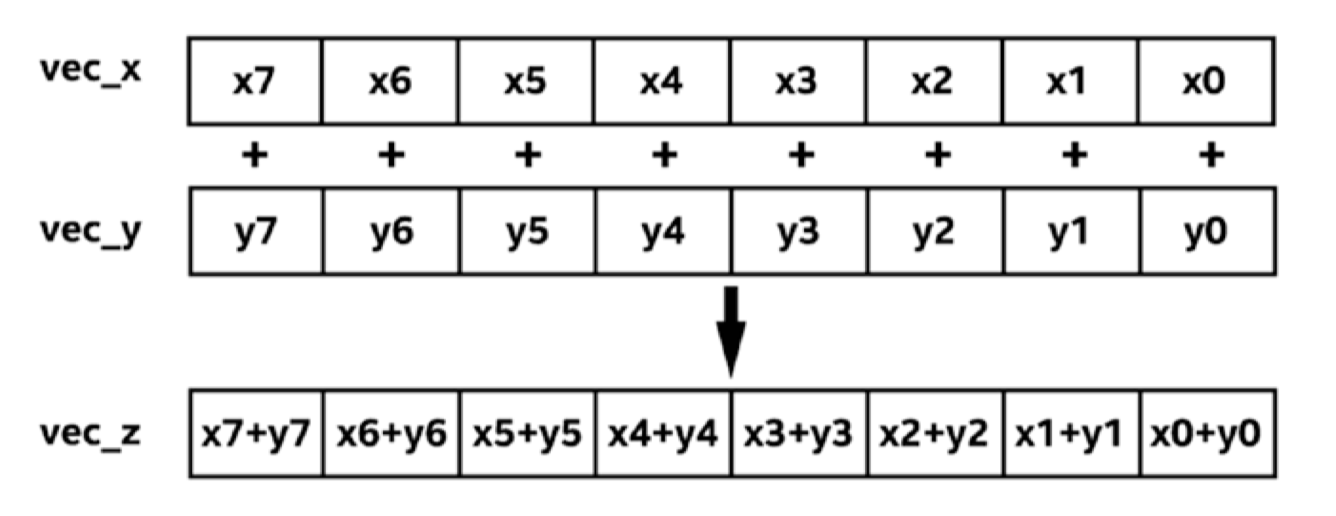
\includegraphics[width=0.9\textwidth]{figs/F11.11.png}
	\caption{\textit{具有八位数据并行性的 SIMD 添加 }}
\end{figure}

在提供SIMD硬件的设备上,我们可以考虑进行向量加法运算,例如,对八元素向量进行加法运算,如图11-11所示。

此示例中的向量加法可以使用向量硬件在单个指令中执行,与该 SIMD 指令并行添加向量寄存器 vec\_x 和 vec\_y。

SIMD 类型到向量硬件的这种映射非常简单且可预测,并且任何编译器都可能以相同的方式执行。 
这些属性使得 SIMD 类型对于 SIMD 硬件上的低级性能调整非常有吸引力,
但也带来了成本——代码的可移植性较差,并且对特定架构的细节变得敏感。 SPMD 编程模型的发展是为了应对这些成本。

开发人员期望 SIMD 类型具有可预测的硬件映射属性,
这正是通过两种不同的语言功能干净地分离向量的两种解释至关重要的原因:如果开发人员使用一种便利类型,
希望其表现得像 SIMD 类型,他们很可能会这样做 正在反对编译器优化,并且可能会看到性能低于希望或预期的性能。

\subsection{总结}
编程语言中的术语向量有多种解释,在编写高性能和可扩展的代码时,理解特定语言或编译器所围绕的解释非常重要。 
SYCL 的构建理念是,源代码中的向量类型是Work-Items本地的便利类型,
并且编译器跨Work-Items进行的隐式向量化映射到硬件中的 SIMD 指令。 
当我们(在极少数情况下)想要编写直接映射到矢量硬件的代码时,
我们应该查看供应商文档,在某些情况下还应该查看 SYCL 的扩展。 
大多数应用程序应该假设Kernel将跨Work-Items进行矢量化,这样做会利用 SPMD 的强大抽象,
它提供了易于推理的编程模型,并提供了跨设备和架构的可扩展性能。

本章描述了 marray 接口,当我们想要操作类似类型的数据分组(例如,具有多个颜色通道的像素)时,它提供了开箱即用的便利。 
此外,我们还讨论了遗留的 vec 类,它可以方便地表达某些模式(使用 swizzles)或优化(使用加载/存储和后端互操作性)。